\section{Implementation}
%how to validate implementation
\noindent{\bf Persistent memory hardware} We emulate persistent memory using volatile DRAM memory. NVMs are slower than DRAM, so we account for 
slow NVM latency using memory throttling. The modern CPUs allow us to configure the duty cycle value in the memory channel. We use that
facility to throttle the bandwidth of the DRAM memory device, reducing the bandwidth and latency of the DRAM reads/writes. 

\noindent{\bf Persistent containers}
We use persistent data-structure implementations of Intel PMDK to model our persistent containers. The PMDK's goal is not to 
create persistent containers. Hence we had to wrap some of their persistent memory data-structures to fit our container model.
e.g.: Wrapping B+tree with map interface.

\noindent{\bf Data Replication}

We use log replication system software layer called cyclone~\cite{cyclone} for our data replication. Cyclone implements 
state machine replication with Raft as the consensus protocol. Cyclone network transports use highly optimized 
userspace Intel's data plane development kit (DPDK) transport stack. Due to this, we had to port YCSB benchmark to
use same DPDK transport for performance reasons.

\section{Implementation}



\section{Evaluation}
%evaluate performance
We evaluate a prototype version of Blizzard to understand the initial peformance characteristics of the proposed
system. Specifically, we seek to answer the following question -- ``What is the cost of reliable data-structures of
Blizzard comapred to state of the art system storage stacks?. ``

To this end we evaluate the performance of reliable persistent map data structure of Blizzard to a state of the art
key-value store implementation. We describe each of them below.

\noindent{Blizzard persistent-map}
This is a persistent B+tree structure that works with our operations replication layer. The internal nodes
store 64 keys, and maintain sorted ordering at all times. We use copy-on-write (COW) crash consistency 
semantics -- we create a new subtree and copy the data over, whenever we encounter a internal node split. 
We then switch the consistent view of the tree to new subtree using an atomic CAS primtive. 
\noindent{RocksDB}
RocksDB is an open source persistent storage engine by Facebook. It is being used by number of production quality
applications as their persistent storage stack. The key data-structure supporting RocksDB is, log-structured merge
tree (LSM) ~\cite{lsm}. LSM workaround the slow writes of SSD storage device by buffering them on the main memory.
We point both write-ahead-log (WAL) and storage structures (SSTables) of RocksDB to use NVM memory.

\noindent{workload}
We use a YCSB like workload to benchmark these different backends. The client is remote to the replication
cluster and uses DPDK network stack to communicate with the master node. The operations are key-value updates and
reads with configurable ratios between them. The client uses an asynchronous message semantics so that we can
load the target backend server with enough requests.

%testbed
We use a three machine nodes connected with ethernet networking hardware as our testbed. We use real NVM hardware
in our test platform. The workload generator/client sits in a separate node. We list the hardware configuration of
our test bend in ~\autoref{testbed}
\begin{table}[h!]
	\centering
	\begin{tabular}{l|l}
		\hline
		CPU & 1.2 Ghz, 96 cores over 2 NUMA sockets \\
		Replicas & 3 replicas. Single master \\
		Network & 100G ethernet LAN \\
		Network-stack & Intel DPDK \\
		DRAM & 256 GB \\
		NVRAM & 1 TB \\
	\end{tabular}
	\caption{Evaluation testbed details}
	\label{testbed}
\end{table}

%result analysis

\begin{figure}[tbp]   
	\centering
	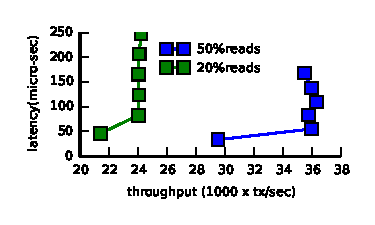
\includegraphics[width=\linewidth]{plot/rocksdbcompare.pdf} 
	\caption{\small RocksDB throughput latency numbers under different read/write ratios. The WAL and the SSTables are placed on NVM. The replication\_factor=1} 
	\label{fig:pmemkv} 
\end{figure}

\begin{figure}[tbp]   
	\centering
	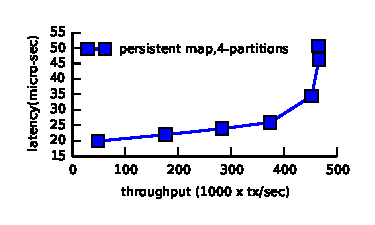
\includegraphics[width=\linewidth]{plot/bliztree-partition.pdf} 
	\caption{\small B-tree based persistent map with 4 partitions/executor threads. We replicate each update over 3 nodes} 
	\label{fig:pmemkv} 
\end{figure}








%future work
Furthermore,we plan to evaluate our system with a real application workload. In this experiment setup, we try to understand the costs
and benefits involved while using a reliable persistent containers as the basic application's peristent storage abstraction.
We looked in to porting a ``Hackernews`` like web-application to use Blizzard data-structures. The application named Lobsters
~\cite{lobsters} among others, maintain two key tables named ``posts`` and ``votes``. The first table stores the 
title,url,etc related to particular post and the latter stores the individual vote counts for a given post. The original
Lobsters application uses an inner join to between these two tables to derive the output table that has top-most K posts
by votes. We identify that this read pattern can be effectively supported using a more natural in-memory data strucutre --
persistent priority queue. We are working towards that.


\section{Project Goals}
%project goals description
We have identified the following goals for our project.
\begin{itemize}
    \item {\bf The 75$\%$ goal:} 1) Porting a Tree (range lookup) and Map ( point lookup) data structure as a reliable persistent containers. 2) Implementing client side library routines to interact with those containers over the network. 
    \\ \\
    At first, we spend couple weeks exploring different ideas. Our original thought was to extend the database indexing process to the non-volatile memory. However, we realized that data replication actually introduces large amount of overhead to the system. Therefore, we switched to designing a reliable protocol for database data. For the 75$\%$ goal, we utilize the pmem library to emulate the non-volatile memory and successfully port the client side library with containerized service.
    \\
    \item {\bf The 100$\%$ goal:} 1) Port YCSB benchmark to work with our containers. 2) Port a state of the art kv-store (RocksDB). 3) Using ported YCSB benchmark client, report numbers for Blizzard containers and competing state of the art. ( RocksDB ).
    \\ \\
    YCSB is a comprehensive test benchmark provided by Yahoo open source. It is mainly coded in Java. Users can create a interface in YCSB to interact with the actual DBMS and the performance will be tested through the interface. The major issue of this goal is that YCSB is mostly in Java, but our implementation is in C++. Therefore, for this goal, we utilized a already implemented driver from Pelaton to interact with the YCSB testing benchmark. 
    \\
    \item {\bf The 125$\%$ goal:} Extend and PMWCAS to support reliability. This include design of the primitive as it is not straight forward at this point to design it.
    \\ \\
    We have learned PMWCAS and tried to port it into our framework, but due to its complexity of dealing with multi-word concurrency update, we are not able to port it into our prototype. 
\end{itemize}



			\section{Related Work}

			PMWCAS~\cite{pmwcas} is a programming primtive that supports both persistency and multiword updates.
			It extends well known CAS pritmive with multiword support while supporting same all or nothing
			programming semantics of CAS. Furthermore, it extends the CAS to be persistent memory aware by
			adding support for durability semantics ( fences and cache-line flushes).

			Intel PMDK~\cite{pmdk} provides persistent memory aware data-structures. But they lack the reliability semantics.

			Mojim from UCSD, in order to achieve data reliability and availability under large scale condition, it uses two tier architecture in which the primary tier contains a mirrored pair of node and the secondary tier contains one or more secondary backup nodes with weakly consistent copies of data. Mojim protocol provides an extra layer of redundancy so that users are able to specify whether they want to ensure strong or weak consistency between primary node and backup node. Though the Mojim shows good performance in terms of latency and throughput, it does not scale well under high concurrency. When the number of users is high, it suffers from reduced latency and throughput. 

\section{Conclusion}
In this project, we successfully design a non-volatile memory based storage stack Blizzard. The proposed stack uses non-volatile memory and modern networking system to provide a fast and also reliable persistent data storage. In our work, we show that even though logical data replication is not common in non-volatile memory domain, with careful adoption, we are able to achieve good performance. In addition, we design a prototype in our work, which shows good throughput and latency compared to previous work. We believe that the system can be adopted with other real world applications and also achieve good performance. 

\section{Future Work}
In this work, the idea is only tested in a basic prototype, but the real world application may introduce more random behaviors compared to an idealized prototype. Therefore, the next step is that we can extend our prototype to real world application that actually performs select or join operations. We have made some progress on Lobsters web app which is similar to Hackernews, but we expect to extend our framework and test it out on other real world applications. 

In this work, we did not get a chance to evaluate the PMDK physical replication implementation. In this future, we will think about how to comprehensively evaluate the physical replication implementation's performance. 

Lastly, we could also work on the PWMCAS porting in the future to finish the 125$\%$ goal.
